\input{../../../.preambles/02-lab_work}
\newgeometry{top=1.5cm, bottom=1.5cm, left=1cm, right=1cm}
\begin{document}
    \begin{table}[h!]
        \center
        \begin{tabular}{|C{.5}|C{.2}|C{.25}|}
            \hline
            \multicolumn{1}{|c|}{\multirow{4}{*}{Лабораторная работа № 2}} &
            Студент, группа & {{ student }}, Ф-369 \\ \cline{2-3}
            & Дата выполнения & 22.03.2013 \\ \cline{2-3}
            & Подпись &  \\ \cline{2-3}
            Логические устройства& Дата отчёта & \\ \cline{2-3}
            & Оценка &  \\ \cline{2-3}
            & Подпись &  \\ \hline
        \end{tabular}
    \end{table}

    \emph{Цель работы:} научиться составлять схемы простейших устройств,
    основанных на базовых логических элементах, в программной среде
    \emph{Quartus}.
    
    \subsection{Двухбитный сумматор}
    \vspace{-1em}
    
    \begin{table}[!ht]
        \begin{minipage}{.5\textwidth}
            Двухбитный сумматор -- устройство, складывающее два числа от 0 до
            3. Фрагмент его таблицы истинности приведен в таблице
            \ref{tab_adder}, где \( A_{0,1} \) -- биты числа \( A \),
            \( B_{0,1} \) -- биты числа \( B \), \( C_{0,1,2} \) -- биты
            полученного числа \( C \); в таблице опущены значения входных
            чисел, при которых получается уже показанный результат на выходе.
            Схема сумматора и его временная диаграмма при \( A \) и \( B \)
            постепенно меняющихся от 0 до 3 представлены на рисунке
            \ref{pic_adder}.
        \end{minipage}\hspace{2em}
        \begin{minipage}{.45\textwidth}
            \caption{Фрагмент таблицы истинности сумматора}
            \label{tab_adder}
            \begin{tabular}{|*{7}{C{.1}|}} \hline
                \( A_1 \) & \( A_0 \) & \( B_1 \) & \( B_0 \) & \( C_2 \) &
                \( C_1 \) & \( C_0 \) \\ \hline
                0 & 0 & 0 & 0 & 0 & 0 & 0 \\[-.5em]
                0 & 0 & 0 & 1 & 0 & 0 & 1 \\[-.5em]
                0 & 0 & 1 & 0 & 0 & 1 & 0 \\[-.5em]
                0 & 0 & 1 & 1 & 0 & 1 & 1 \\[-.7em]
                & & & \( \cdots \) & & & \\[-.7em]
                0 & 1 & 1 & 1 & 1 & 0 & 0 \\[-.7em]
                & & & \( \cdots \) & & & \\[-.7em]
                1 & 0 & 1 & 1 & 1 & 0 & 1 \\[-.7em]
                & & & \( \cdots \) & & & \\[-.7em]
                1 & 1 & 1 & 1 & 1 & 1 & 0 \\ \hline
            \end{tabular}
        \end{minipage}
    \end{table}
    
    \vspace{-1em}
    \begin{figure}[h!]
        \center
        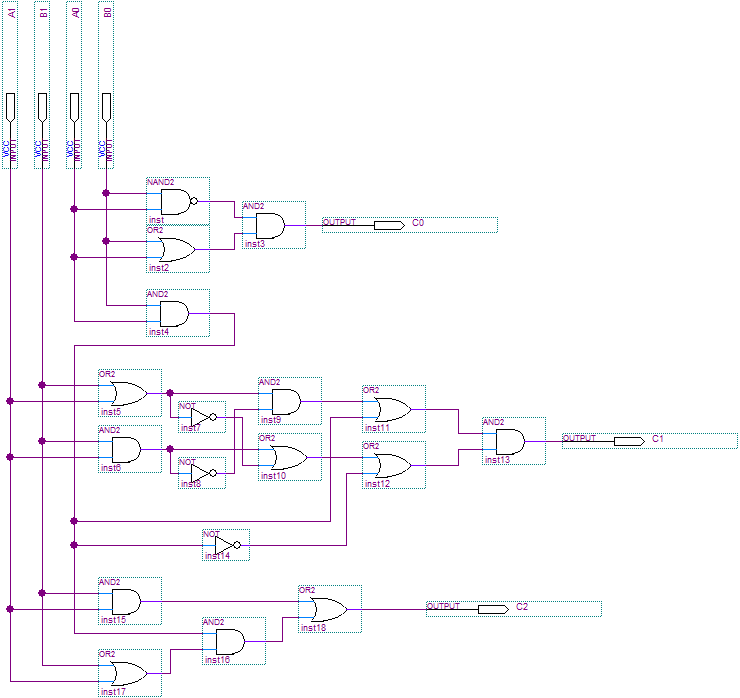
\includegraphics[width=.7\textwidth]{adder} \vspace*{2em}\\
        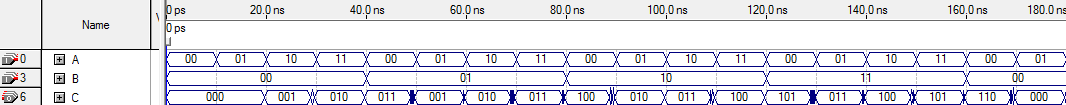
\includegraphics[width=.75\textwidth]{adder_time}
        \caption{Схема сумматора и его временная диаграмма}
        \label{pic_adder}
    \end{figure}
    
    \pagebreak
    
    \subsection{Двухбитный дешифратор}
    
    \begin{table}[!ht]
        \begin{minipage}{.5\textwidth}
            Двухбитный дешифратор -- устройство, подающее на один из своих
            выходов логическую единицу и нули на остальные в зависимости от
            двоичного кода на входе. Его таблица истинности приведена в таблице
            \ref{tab_dc}, где \( A_{0,1} \) -- код на входе, \( D_{0,1,2,3} \)
            -- состояния выходов устройства. Схема дешифратора и его временная
            диаграмма представлены на рисунке~\ref{pic_dc}.
        \end{minipage}\hspace{2em}
        \begin{minipage}{.45\textwidth}
            \caption{Таблица истинности дешифратора}
            \label{tab_dc}
            \begin{tabular}{|*{6}{C{.1}|}} \hline
                \( A_1 \) & \( A_0 \) & \( D_3 \) & \( D_2 \) & \( D_1 \) &
                \( D_0 \) \\ \hline
                0 & 0 & 0 & 0 & 0 & 1 \\
                0 & 1 & 0 & 0 & 1 & 0 \\
                1 & 0 & 0 & 1 & 0 & 0 \\
                1 & 1 & 1 & 0 & 0 & 0 \\ \hline
            \end{tabular}
        \end{minipage}
    \end{table}
    
    \begin{figure}[h!]
        \center
        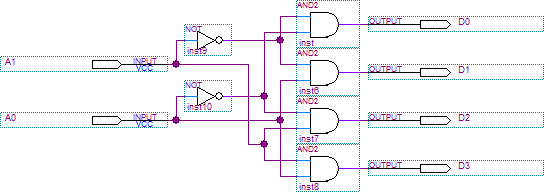
\includegraphics[width=.8\textwidth]{decoder} \vspace*{1em}\\
        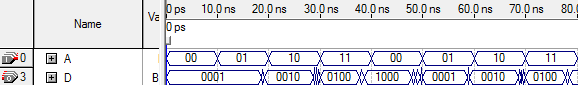
\includegraphics[width=.75\textwidth]{decoder_time}
        \caption{Схема дешифратора и его временная диаграмма}
        \label{pic_dc}
    \end{figure}
    
    \subsection{Трехбитный счетчик на JK-триггерах}
    
    Трехбитный счетчик -- устройство, на выходы которого подается двоичный код,
    увеличивающийся на единицу при очередном такте синхроимпульса; после
    состояния ``111'' идет состояние ``000'' -- сброс счетчика. Счетчики могут
    быть основаны на различных элементах, в данном случае -- на JK-триггерах.
    На входы \emph{J} и \emph{K} первого триггера подается логическая единица,
    на последующие -- конъюнкция двух предыдущих выходов, т.е. на второй
    триггер идет \( Q_0 \wedge 1 = Q_0 \), на третий -- \( Q_1 \wedge Q_0 \) и
    т.д.
    
    Схема и временная диаграмма счетчика приведены на рисунке
    \ref{pic_counter}.
    
    \begin{figure}[h!]
        \center
        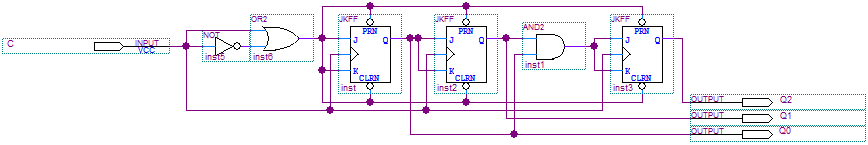
\includegraphics[width=\textwidth]{counter} \vspace*{1em}\\
        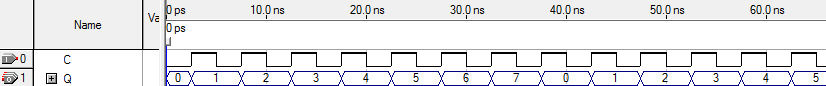
\includegraphics[width=.9\textwidth]{counter_time}
        \caption{Схема счетчика и его временная диаграмма}
        \label{pic_counter}
    \end{figure}
    
    \pagebreak
    
    \subsection{Двухбитный мультиплексор}
    \vspace{-2em}
    \begin{table}[!ht]
        \begin{minipage}{.6\textwidth}
            Двухбитный мультиплексор -- устройство, соединяющее один из своих
            входов с выходом в зависимости от управляющего сигнала. Его таблица
            истинности приведена в таблице \ref{tab_mux}, где \( A_{0,1,2,3} \)
            -- состояния входов, \( D_{0,1} \) -- управляющий сигнал, \( C \)
            -- состояние выхода. Схема мультиплексора и его временная диаграмма
            представлены на рисунке \ref{pic_mux}.
        \end{minipage}\hspace{2em}
        \begin{minipage}{.3\textwidth}
            \caption{Таблица истинности мультиплексора}
            \label{tab_mux}
            \begin{tabular}{|*{3}{C{.25}|}} \hline
                \( D_1 \) & \( D_0 \) & \( C \) \\ \hline
                0 & 0 & \( A_0 \) \\[-.5em]
                0 & 1 & \( A_1 \) \\[-.5em]
                1 & 0 & \( A_2 \) \\[-.5em]
                1 & 1 & \( A_3 \) \\ \hline
            \end{tabular}
        \end{minipage}
    \end{table}
    
    \vspace{-2em}
    \begin{figure}[h!]
        \center
        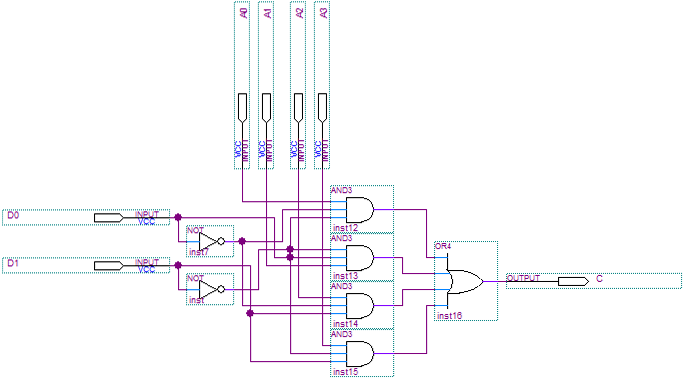
\includegraphics[width=.7\textwidth]{multiplexer} \vspace*{1em}\\
        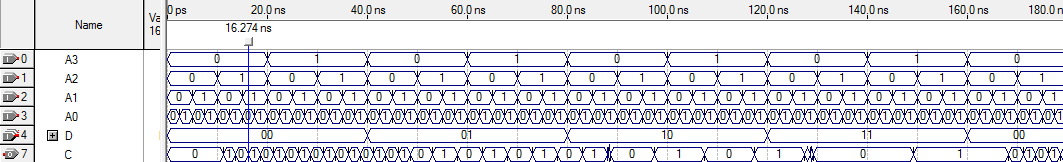
\includegraphics[width=\textwidth]{multiplexer_time}
        \caption{Схема мультиплексора и его временная диаграмма}
        \label{pic_mux}
    \end{figure}
    
    \vspace{-1em}
    \subsection{Четырехбитный сдвиговый регистр на JK-триггерах}
    
    Регистр -- устройство, предназначенное для записи, хранения и
    преобразования информации, представленной в двоичном коде. Четырехбитный
    сдвиговый регистр работает с четырьмя битами информации, сдвигая по сигналу
    \emph{Shift} текущий код влево и записывая в младший бит новое значение со
    входа \emph{data}. Его схема и временная диаграмма со случайными значениями
    на входе \emph{data} приведены на рисунке \ref{pic_reg}.
    
    \begin{figure}[h!]
        \center
        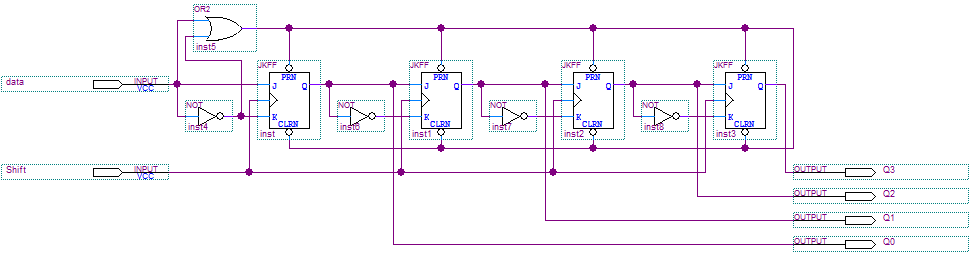
\includegraphics[width=.9\textwidth]{register} \vspace*{1em}\\
        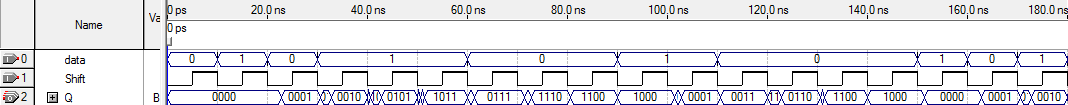
\includegraphics[width=\textwidth]{register_time}
        \caption{Схема регистра и его временная диаграмма}
        \label{pic_reg}
    \end{figure}    
\end{document}
